\begin{frame}
\frametitle{Freiheit der Wissenschaft an der Universität}
selbst einschränkungen in der Wissenschaft
    Zivilklausel
    ethikkommissionen? Rechtlich?
    selbst einschränkungen in der Lehre
    Akkriditionsverfahren
\end{frame}

\subsection*{Zivilklausel}
\begin{frame}
\frametitle{Zivilklausel}
\begin{itemize}
\item Selbstverpflichtung von wissenschaftlichen Einrichtungen ausschließlich für zivile Zwecke zu forschen. \cite{ZivKlausel}
\item Die erste Zivilklausel trat 1986 an der Universität Bremen in Kraft.
\end{itemize}

\end{frame}

\begin{frame}
\frametitle{Liste mit Hochschulen mit einer Zivilklausel}
\begin{multicols}{2}
\begin{itemize}
\item TU Berlin
\item Uni Bremen
\item Uni Konstanz
\item TU Dortmund
\item Uni Oldenburg
\item TU Ilmenau
\item Uni Tübingen
\item Uni Rostock
\item HS Bremen
\item HS Bremerhaven
\item TU Darmstadt
\item Uni Göttingen
\item Uni Frankfurt am Main
\item Uni Münster
\end{itemize}
\end{multicols}

\end{frame}

\begin{frame}
\frametitle{Pro und Contra Zivilklausel}
\tiny{
\begin{table}
\begin{tabularx}{\linewidth}{>{\parskip1ex}X@{\kern4\tabcolsep}>{\parskip1ex}X}
\toprule
\hfil\bfseries Pros
&
\hfil\bfseries Cons
\\\cmidrule(r{3\tabcolsep}){1-1}\cmidrule(l{-\tabcolsep}){2-2}

%% PROS, seperated by empty line or \par
Der Zwei-plus-Vier-Vertrag besagt, \glqq dass von deutschem Boden nur Frieden ausgehen wird. \grqq \par
Universitäten könnten Teil der Kriegsmaschinerie werden. Bzw. sind es schon.\par
Auch ohne Zivilklausel ist die Wissenschaft nicht frei und wird von den Interessen der Industrie gelenkt.\par
Wissenschaft hat das Potenzial, großen Schaden anzurichten. (Atombombe) \par
Die Zivilausel ist \glqq ein Merkmal der Universität, das man auch nach außen tragen kann.\grqq \cite{ohbtaz}\par
\dots \par

&

%% CONS, seperated by empty line or \par
Einige Klauseln verstoßen gegen die im Grundgesetz garantierte Freiheit von Forschung und Lehre. \cite{JKrause} \par
Eine Zivilklausel ist Realitätsfern. (Dual use ist nicht zu vermeiden) \par
Militärforschung hat immer wieder großen Nutzen für die Zivilnutzung erbracht. \par
Eine Zivilklausel schreckt mögliche private Investoren ab. \par
\dots \par
\\\bottomrule
\end{tabularx}
\caption{Pro und Contra Zivilklausel}
\end{table}
}
\end{frame}

\subsection*{Situation an der Universität Bremen}
\begin{frame}
2011 wurde die Zivilklausel der Uni Bremen erfolgreich verteidigt.


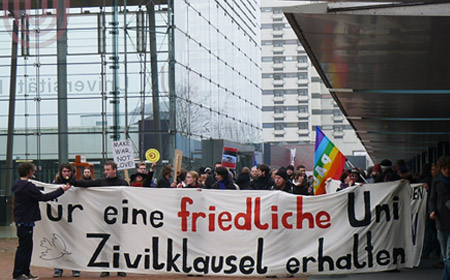
\includegraphics[scale=0.5]{images/zivilklausel.jpg}
{\tiny{Quelle: http://jetzt.sueddeutsche.de/upl/images/user/qu/quentin-lichtblau/text/regular/901608.jpg}}

\end{frame}

\subsection*{Akkriditionsverfahren}
\begin{frame}
Akkriditionsverfahren dienen der Qualitätssicherung von Studiengängen.
\end{frame}

\begin{frame}
Kritik:
\glqq Die Akkreditierung in Deutschland ist teuer, bürokratisch, langsam, ineffizient, rechtlich zweifelhaft und autonomiefeindlich.\grqq Professor Dr. Bernhard Kempen Präsident des DHV
\end{frame}

\begin{frame}
Das Fach Informatik Bachelor der Universität Bremen wurde  
akkreditiert am 11.10.2006 durch die ASIIN
\end{frame}

\subsection*{Ethikkommissionen}
\begin{frame}
Ethikkommisionen dienen der Beurteilung der Forschungsvorhaben, die an Lebewesen durchgeführt werden, aus ethischer, rechtlicher und sozialer Sicht sowie der Schutz des Individuums vor den Folgen der (klinischen) Forschung am Lebewesen.

\end{frame}

\begin{frame}
An der Universität Bremen: Aufgabe der Ethikkommission ist
1.     die Prüfung und Beurteilung der ethischen Zulässigkeit von Forschungsvorhaben, die Untersuchungen an Menschen, an vom Menschen genommenen Proben oder Forschungen mit personenbezogenen Daten von Probanden oder Patienten beinhalten,
2.     die Beratung und Verabschiedung von Grundsätzen der ethischen Bewertung von Tierversuchen.
Quelle: http://www.ethikkommission.uni-bremen.de/EthikO.htm

\end{frame}



